\documentclass[11pt]{article}

\usepackage[a4paper,margin=1in]{geometry}
\usepackage{amsmath,amssymb}
\usepackage{booktabs}
\usepackage{graphicx}
\usepackage{longtable}
\usepackage{tabularx}
\usepackage{array}
\usepackage{ragged2e}
\usepackage{hyperref}
\usepackage{url}
\usepackage{xcolor}

\graphicspath{{../figures/}}
\newcolumntype{Y}{>{\RaggedRight\arraybackslash}X}
\newcolumntype{P}[1]{>{\RaggedRight\arraybackslash}p{#1}}

\hypersetup{
  colorlinks=true,
  linkcolor=blue!45!black,
  citecolor=blue!45!black,
  urlcolor=blue!45!black
}

\title{\textbf{Research Artifact and Reproducibility Package:\\
Objective Clock Bases from Redundant Records}}
\author{Davut Emre Tasar}
\date{Artifact report frozen on 2026-06-21}

\newcommand{\artifacttitle}{Research Artifact and Reproducibility Package: Objective Clock Bases from Redundant Records}

\begin{document}
\maketitle

\begin{abstract}
This report documents the public research artifact \emph{\artifacttitle}.
The artifact investigates a narrow question at the boundary between quantum
Darwinism, redundant records, and relational clock structure.  Here a
\emph{clock} is not a laboratory timing device; it is a candidate quantum
subsystem whose basis labels are interpreted as possible time labels inside a
larger quantum state.  The central question is: if records make such a clock
basis objective, what additional structure is required to recover event order
and temporal orientation?  The package supports a deliberately limited answer.
Fixed-partition redundant records can identify an objective record basis under
assumptions already treated in the literature, but that basis is not a physical
time line by itself.  Persistent physical trajectories are chains in the
record-dominance poset.  Branching linear extensions are scheduler
totalizations, not physical histories.  Temporal orientation also requires an
anchor beyond redundancy alone.  The artifact includes proof notes, exact
classical experiments, local quantum-readiness checks, a preregistered
four-qubit IBM Quantum illustration on \texttt{ibm\_kingston}, a locked raw
hardware analysis, a secondary readout-mitigation check, a claim-evidence
matrix, and a reproducibility archive.
\end{abstract}

\tableofcontents

\section{Why This Artifact Exists}

The motivating problem comes from quantum foundations rather than from
timekeeping engineering.  Quantum Darwinism and environment-as-a-witness
arguments explain how many environment fragments can carry redundant
information about selected system properties
\cite{OllivierPoulinZurek2004,BlumeKohoutZurek2006,Zurek2009,Korbicz2021}.
Objective-past work asks how redundant records can support agreement about
histories \cite{RiedelZurekZwolak2016}.  Fu's uniqueness theorem clarifies a
fixed-partition setting in which a redundantly imprinted observable is unique,
while also leaving partition dependence as a boundary \cite{Fu2021}.

Those results motivate a sharper quantum-clock question.  Suppose a larger
quantum state contains a candidate clock subsystem \(C\), and suppose
independent fragments \(R_1\) and \(R_2\) redundantly record the labels of
\(C\).  Has that recovered time, or only an objective label basis?  The artifact
tests the latter view.  Agreement on the displayed alternatives is not yet
agreement on a physical history.  A list of objective quantum snapshots still
leaves three distinct tasks:
\begin{enumerate}
  \item identify the recorded basis;
  \item order the recorded snapshots into persistent trajectories;
  \item orient the order as earlier-to-later rather than later-to-earlier.
\end{enumerate}
The artifact was built to keep these tasks separate.  This matters because a
single mathematical object, such as a total ordering of snapshots, can look like
a time line while failing the physical persistence condition.  The central
correction made during the work is that linear extensions of a branching
record-poset are not physical time lines.  They are merely total schedules
compatible with a partial order.  A physical scalar time is available only when
the relevant snapshots lie on one chain.

For a non-specialist reader, the simplest analogy is a book with copied page
notes.  The candidate clock label is like a page number.  The record fragments
are like independent notes copied from the page.  Agreement between notes can
make the page number objective, but it does not prove that the pages form one
story, that the story has no branches, or that the reading direction has been
selected by the records themselves.  The artifact formalizes this gap in a
small quantum setting.

\section{Experimental Quantum System}

The bounded hardware illustration uses four logical qubits.  \(C\) is the
candidate clock-label subsystem, \(S\) is a companion system qubit used in the
global coherence witness, and \(R_1,R_2\) are independently accessible record
fragments.  The GHZ state tests redundant \(Z\)-basis records of \(C\) in
\(R_1\) and \(R_2\).  A matched dephased-control state preserves those local
\(Z\) records but removes global \(X\) coherence.  This is the operational
reason for measuring both local \(Z\)-record correlations and global
\(XXXX\)-type coherence witnesses.

\section{Scientific Boundary}

The artifact is not a claim that fixed-partition basis uniqueness is new.  It
treats pointer-basis and redundant-imprint results as background
\cite{Zurek1981,Fu2021}.  It is also consistent with the objective-past program
of Riedel, Zurek, and Zwolak, where redundant records of histories support
objective past structure \cite{RiedelZurekZwolak2016}.  The contribution here is
the separation package:
\begin{itemize}
  \item basis objectivity is not scalar time;
  \item scalar time requires a chain condition in the record-dominance poset;
  \item orientation requires an external or physical anchor;
  \item record capacity and no-go examples make the limits explicit;
  \item the IBM Quantum run is a bounded illustration, not the proof base.
\end{itemize}

\section{Concept Primer}

\begin{table}[htbp]
\centering
\begin{tabularx}{\textwidth}{@{}P{0.26\textwidth}Y@{}}
\toprule
Concept & Working meaning in the artifact \\
\midrule
Clock basis &
A basis of a candidate quantum subsystem whose labels are possible time labels;
it is not a literal clock face or external timing device. \\
Objective basis &
A basis whose alternatives are redundantly recoverable from independently
accessible record fragments under a fixed admissible partition. \\
Record signature &
The tuple of record values associated with a snapshot.  In the binary examples,
this is a string such as \(00\), \(10\), or \(11\). \\
Record-dominance poset &
The partial order induced by persistence: one snapshot can follow another only
when existing records are not lost. \\
Chain &
A totally ordered subset of the poset.  Chains are the candidate persistent
trajectories. \\
Linear extension &
Any total ordering compatible with the poset.  In a branching poset, this is a
scheduler artifact, not a physical trajectory. \\
Scalar time identifiable &
The relevant snapshots form one non-duplicated chain, so a one-dimensional
timeline can visit all snapshots without record loss. \\
Orientation anchor &
Extra structure that decides which direction of a chain is earlier-to-later. \\
\bottomrule
\end{tabularx}
\caption{Non-specialist vocabulary used throughout the artifact.}
\end{table}

\begin{table}[htbp]
\centering
\begin{tabularx}{\textwidth}{@{}P{0.24\textwidth}P{0.31\textwidth}Y@{}}
\toprule
Everyday analogy & Quantum object & Interpretation \\
\midrule
Page number &
\(C\), the candidate clock-label subsystem &
The label we are tempted to interpret as time. \\
Independent copied notes &
\(R_1\) and \(R_2\), record fragments &
Separate fragments should recover the same label. \\
Readable story &
Chain in the record-dominance poset &
A timeline cannot jump between incompatible branches. \\
Reading direction &
Orientation anchor &
Records can show connection without selecting earlier-to-later. \\
Hidden binding across copies &
Global coherence witness &
This is a quantum witness distinct from local record readability. \\
\bottomrule
\end{tabularx}
\caption{Plain-language map from the analogy to the quantum model.}
\end{table}

\section{Related Work and Positioning}

The artifact sits near three established literatures.  First, environment as a
witness and quantum Darwinism explain how many environment fragments can carry
redundant information about selected system properties
\cite{OllivierPoulinZurek2004,BlumeKohoutZurek2006,Zurek2009}.  Second,
spectrum broadcast structure and strong quantum Darwinism formalize stronger
notions of objectivity and independence
\cite{KorbiczHorodeckiHorodecki2014,HorodeckiKorbiczHorodecki2015,LeOlayaCastro2019,Korbicz2021}.
Third, relational-clock and timeless formulations show why time should not be
introduced carelessly as an external primitive \cite{PageWootters1983}.

The narrow novelty is not that redundancy can select a basis.  Fu's uniqueness
result already addresses uniqueness of the observable leaving redundant
imprints within a fixed subset of partitions, while also emphasizing ambiguity
under different partitions \cite{Fu2021}.  The artifact instead asks what is
still missing after such a basis-level result is granted.  The answer is order
and orientation.

\section{Artifact Architecture}

The repository is organized as a gated research pipeline.  Each stage writes
tracked artifacts with SHA-256 manifests where appropriate.  Raw hardware
payloads are write-once and secret-free.  QPU execution is downstream of the
theory and classical checks.

\begin{center}
\begin{tabularx}{\textwidth}{@{}P{0.12\textwidth}P{0.25\textwidth}Y@{}}
\toprule
Gate & Role & Representative evidence \\
\midrule
G0--G1 & Repository and theorem primitives &
\path{results/processed/T101_chain_verification.json},
\path{results/processed/T103_capacity.json}. \\
G2 & Classical C0--C5 experiments &
Basis landscape, order catalog, noise phase diagram, assumption failures, exact
GHZ analysis. \\
G3 & Local quantum readiness &
Circuit manifest, Aer noise sweep, backend-derived local twin. \\
G4 & Frozen preregistration &
\path{docs/PREREGISTRATION_FROZEN.md} and the frozen circuit packet. \\
G5 & Hardware observation &
One completed IBM run on \texttt{ibm\_kingston}; raw H502 primary analysis and
H503 secondary mitigation. \\
G6 & Interpretation and packaging &
Claim-evidence matrix, final decision, reproducibility archive. \\
\bottomrule
\end{tabularx}
\end{center}

\begin{center}
\begin{tabularx}{\textwidth}{@{}P{0.16\textwidth}P{0.35\textwidth}Y@{}}
\toprule
Code family & Meaning & Example \\
\midrule
\texttt{T} & Theorem and property checks & \texttt{T101} verifies the chain criterion. \\
\texttt{C} & Classical or exact computational experiments & \texttt{C1} tests basis ambiguity. \\
\texttt{Q} & Local quantum-readiness checks & \texttt{Q302} stress-tests the protocol in simulation. \\
\texttt{H} & IBM hardware execution and analysis & \texttt{H501} is the QPU job; \texttt{H502} is raw analysis. \\
\texttt{A} & Audit, interpretation, and packaging & \texttt{A603} records the reproducibility archive. \\
\texttt{G} & Workflow gates & \texttt{G2} means classical experiments are complete. \\
\bottomrule
\end{tabularx}
\end{center}

\section{Core Theoretical Result}

The record signatures induce a partial order: a later snapshot may contain more
persistent records, but it should not erase records already present.  The
artifact checks the following operational consequence:
\[
  \text{scalar time exists} \quad \Longleftrightarrow \quad
  \text{all relevant nonduplicate signatures form one chain.}
\]
The theorem-check artifact \path{results/processed/T101_chain_verification.json}
reports 272 record codes checked and 188,158 sequences checked with zero
mismatches.  The diamond counterexample is decisive: it has two scheduler
linear extensions and two maximal persistent chains, but no full persistent
scalar order visiting all four snapshots.  This is why the report and README
avoid calling branching linear extensions physical time lines.

\begin{figure}[htbp]
\centering
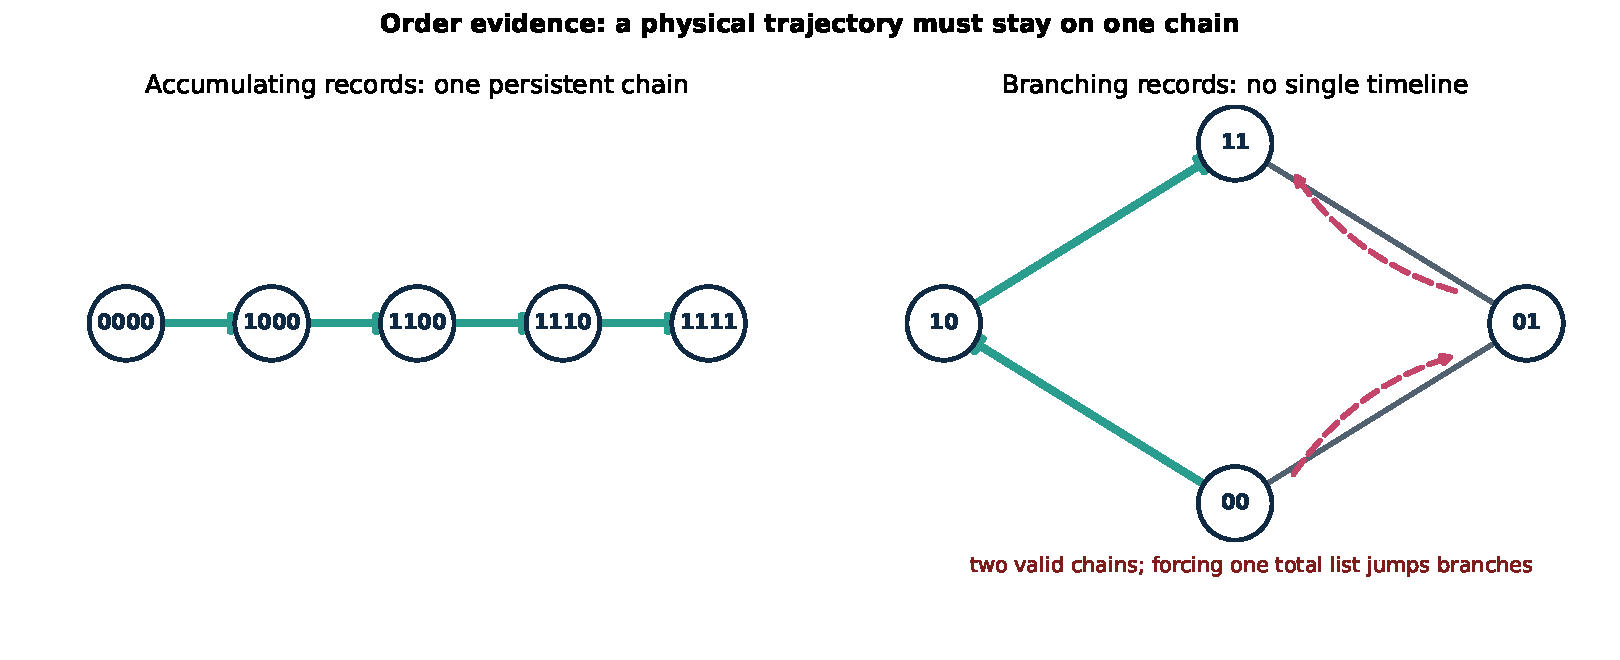
\includegraphics[width=\textwidth]{fig_01_order_chains.pdf}
\caption{How to read record order.  Each circle is a record pattern and each
arrow means that a later pattern can keep all records already present.  The
left example forms one chain, so it can be read as a scalar timeline.  The
right example branches; forcing all nodes into one list would jump between
branches and is not a physical trajectory in this model.}
\end{figure}

\section{Classical Experiments}

\subsection{Basis Landscape}

C1 compares one-record ambiguity with two-record objectivity.  The Bell
one-record example remains maximally ambiguous in the sampled basis landscape,
whereas the GHZ two-record example selects the expected \(Z\)-record basis.
The C1 summary records \(\mathrm{GHZ}_{Z}=1.0\) and
\(\mathrm{GHZ}_{X}=0.0\), while the Bell one-record slice has minimum and
maximum score 1.0.

\begin{figure}[htbp]
\centering
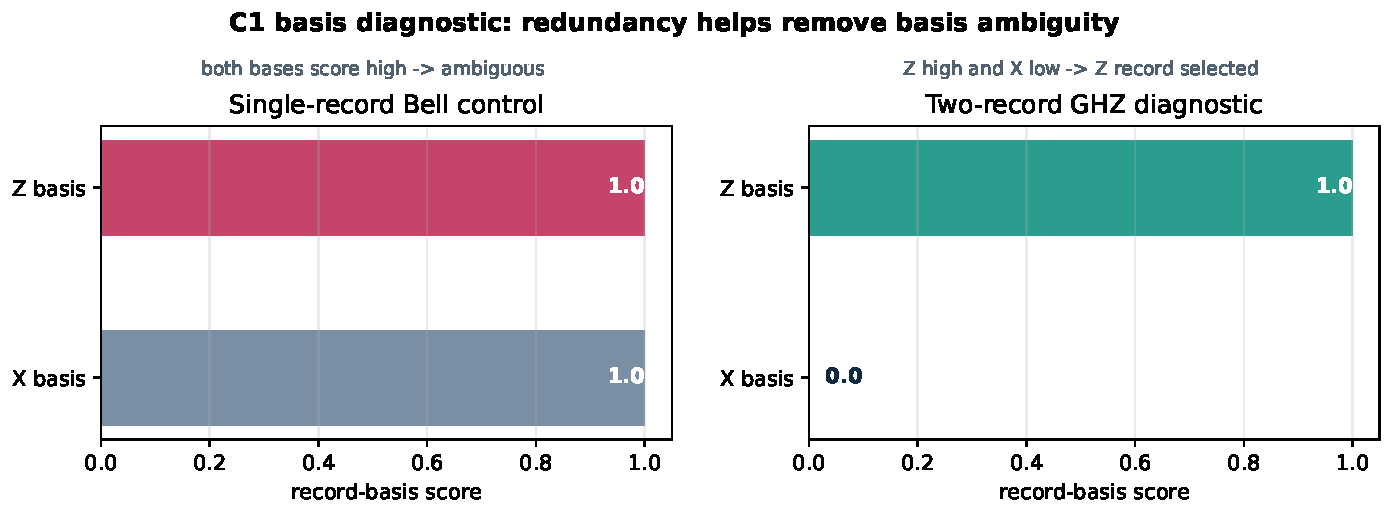
\includegraphics[width=0.96\textwidth]{fig_02_basis_landscape.pdf}
\caption{C1 basis diagnostic.  A single record can make more than one basis look
equally good, which means the basis is ambiguous.  With two GHZ record
fragments, the \(Z\) basis scores high while the \(X\) basis scores low, so the
record basis is selected under the fixed-partition assumptions.}
\end{figure}

\subsection{Record Capacity}

T103 and the C0/C2 family record the capacity constraint for strict-chain
binary records.  With \(E\) binary persistent record coordinates, the maximum
strict-chain length is \(E+1\).  The generated table verifies this from
\(E=0\) through \(E=8\), and the boundary check \(E=N-2\) fails for \(N=2\)
through \(N=9\), as expected.

\begin{figure}[htbp]
\centering
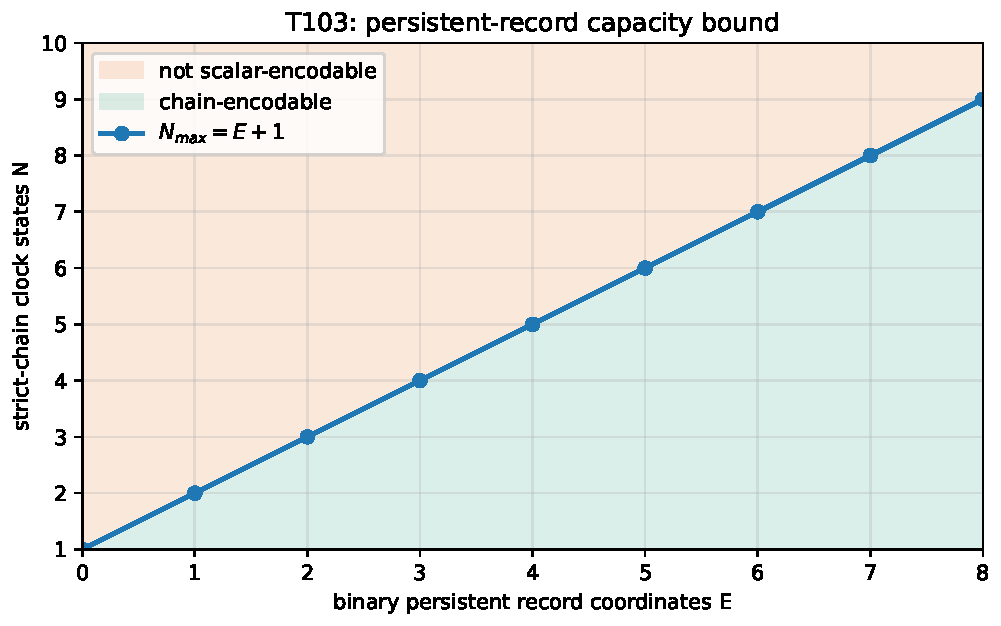
\includegraphics[width=0.86\textwidth]{fig_03_capacity.pdf}
\caption{Persistent record capacity.  A binary record coordinate is like one
persistent switch.  With \(E\) such switches, at most \(E+1\) strict-chain clock
states can be encoded; the shaded region above the line is not scalar
encodable.}
\end{figure}

\subsection{Order Catalog and No-Go Examples}

C2 stores six canonical order examples.  The thermometer case is classified as
\texttt{scalar\_time}.  Diamond and disconnected examples are classified as
branching or partial order.  Duplicate labels are non-identifiable, erasure is
a persistence-violation control, and the orientation-free example records that
direction is not identified.

\begin{table}[htbp]
\centering
\begin{tabular}{@{}ll@{}}
\toprule
Example & Classification \\
\midrule
thermometer & scalar time \\
diamond & branching or partial order \\
disconnected & branching or partial order \\
duplicate & non-identifiable duplicate labels \\
erasure & persistence violation control \\
orientation-free & orientation not identified \\
\bottomrule
\end{tabular}
\caption{C2 order-catalog summary.}
\end{table}

\subsection{Noise and Assumption Stress Tests}

C3 evaluates a 112-cell noise grid and records zero bound violations.  The
recovery boundary moves as expected with bit-flip probability and redundant
copies.  C4 records assumption failures for label permutations, orientation
swaps, unrestricted partitions, single-fragment Bell ambiguity, and diamond
branching.  These examples define where the positive claims stop.

\begin{figure}[htbp]
\centering
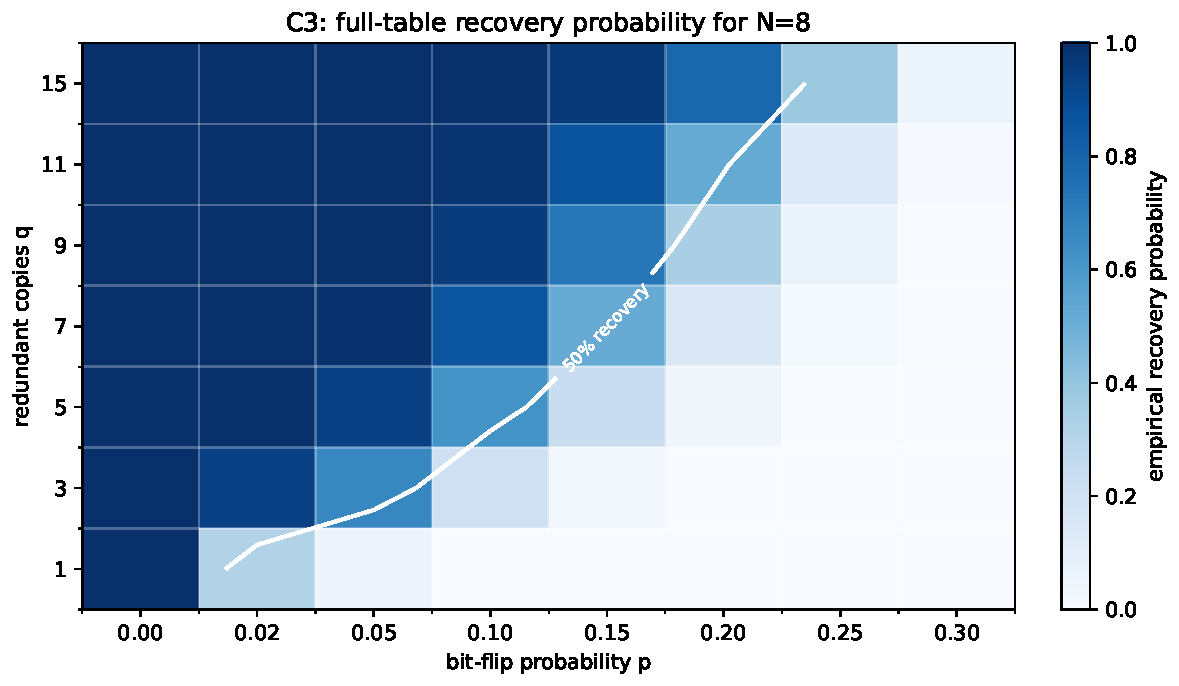
\includegraphics[width=0.88\textwidth]{fig_04_noise_phase.pdf}
\caption{C3 noise phase diagram.  Darker blue cells mean the simulated record
table is recovered more often, pale cells fail more often, and the white
contour marks the approximate 50 percent recovery boundary.  More redundant
copies improve recovery, but no noise result removes the chain and orientation
requirements.}
\end{figure}

\subsection{Exact GHZ and Dephased-Control Check}

C5 checks the exact four-qubit GHZ/dephased-control observables.  Both GHZ and
dephased controls have \(Z\)-record objectivity score 1.0.  The coherence
witness separates them: GHZ has \(\langle XXXX\rangle=1.0\), while the
dephased control has 0.0.  These binary exact values are kept as table evidence
rather than as a standalone publication figure.

\begin{table}[htbp]
\centering
\begin{tabular}{@{}lrr@{}}
\toprule
Observable & GHZ & Dephased control \\
\midrule
\(ZZ_{C,R1}\) & 1.0 & 1.0 \\
\(ZZ_{C,R2}\) & 1.0 & 1.0 \\
\(XX_{C,R1}\) & 0.0 & 0.0 \\
\(XX_{C,R2}\) & 0.0 & 0.0 \\
\(XXXX\) & 1.0 & 0.0 \\
\bottomrule
\end{tabular}
\caption{C5 exact GHZ/dephased-control sanity check.  The control has the same
local \(Z\) records but no global \(X\)-parity coherence.}
\end{table}

\section{Quantum Protocol and Hardware Observation}

The quantum path is deliberately downstream of the theory.  Qiskit is used for
circuit generation and IBM Runtime submission, with a SamplerV2-style bitstring
workflow consistent with the Runtime primitive documentation
\cite{JavadiAbhari2024Qiskit,IBMSamplerV2Docs}.  The preregistered packet
contains 24 circuit instances and 24,576 total shots.  The first submitted
\texttt{ibm\_marrakesh} job was cancelled while queued and is recorded only as
pre-result provenance.  After explicit approval, a pre-result backend amendment
regenerated the dependent artifacts for \texttt{ibm\_kingston}.

\begin{table}[htbp]
\centering
\begin{tabular}{@{}ll@{}}
\toprule
Field & Value \\
\midrule
Backend & \texttt{ibm\_kingston} \\
Job id & \texttt{d8rfasuab0ds73drkaig} \\
Status & \texttt{DONE} \\
Created & 2026-06-20T20:17:55.809388Z \\
Running & 2026-06-20T20:17:57.209474Z \\
Finished & 2026-06-20T20:18:10.354081Z \\
Circuit instances & 24 \\
Observed shots & 24,576 \\
Quantum usage & 9 seconds \\
Secret values recorded & false \\
\bottomrule
\end{tabular}
\caption{Completed H501 hardware observation.}
\end{table}

\begin{table}[htbp]
\centering
\begin{tabular}{@{}lr@{}}
\toprule
Raw H502 metric & Value \\
\midrule
Raw primary inclusion pass & true \\
\(\Delta_{\mathrm{obj}}\) lower confidence bound & 0.8876953125 \\
Minimum \(Z\)-correlation lower confidence bound & 0.9169542107266444 \\
\(\Delta_{\mathrm{coh}}\) lower confidence bound & 0.877685546875 \\
\(\langle XXXX\rangle_{\mathrm{plus}}\) & 0.8955078125 \\
\(\langle XXXX\rangle_{\mathrm{minus}}\) & -0.87744140625 \\
\(\langle XXXX\rangle_{\mathrm{mix}}\) & 0.009033203125 \\
Bootstrap seed & 20260621 \\
Bootstrap replicates & 10,000 \\
\bottomrule
\end{tabular}
\caption{Locked raw hardware analysis.  These are the primary values used for
artifact inclusion.}
\end{table}

\begin{figure}[htbp]
\centering
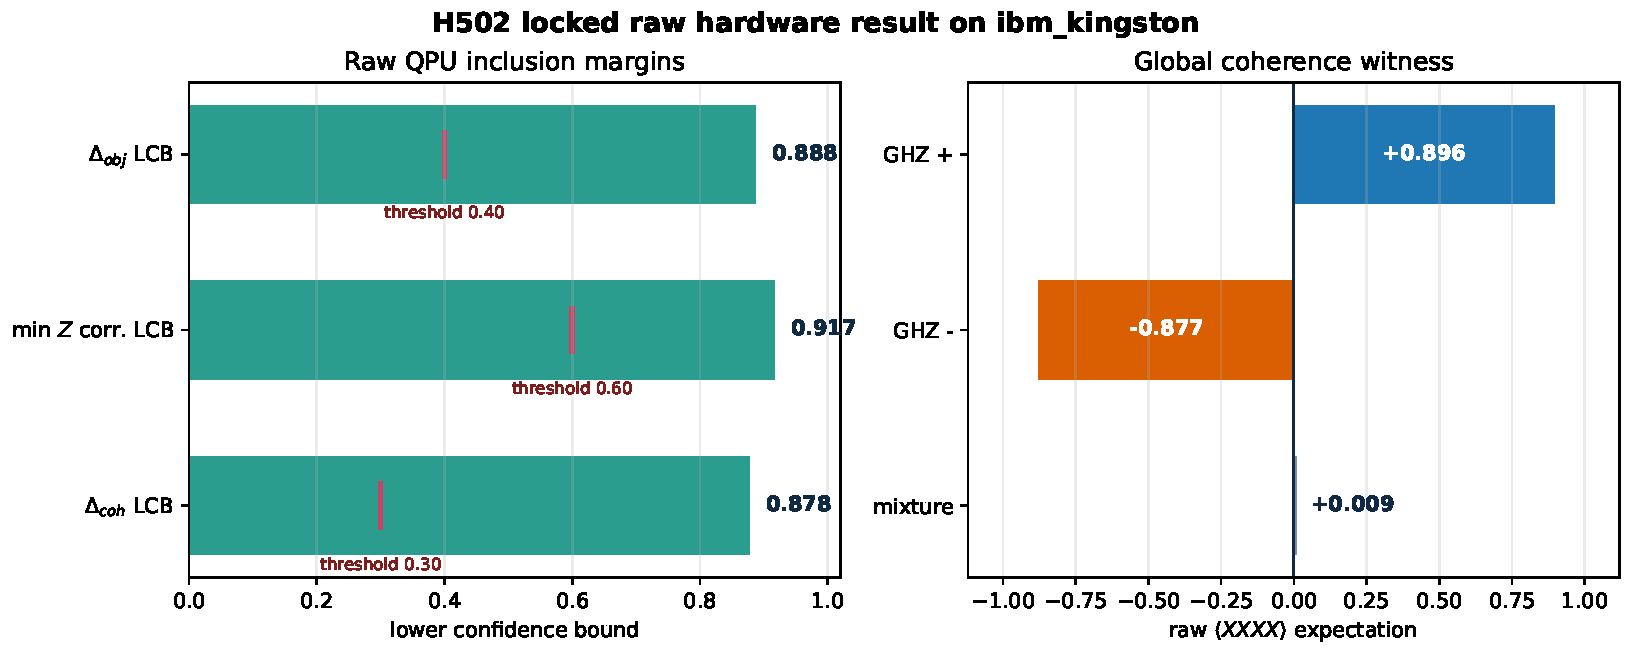
\includegraphics[width=\textwidth]{fig_q3_hardware_summary.pdf}
\caption{H502 locked raw hardware result.  The left panel compares raw lower
confidence bounds with preregistered pass/fail thresholds.  The right panel
shows the measured global \(XXXX\) coherence witness: the GHZ-plus and
GHZ-minus circuits separate from the near-zero mixture.}
\end{figure}

The secondary H503 readout-assignment correction agrees qualitatively with the
raw result.  Its tensor assignment condition number is 1.1172921620957568, with
corrected \(\Delta_{\mathrm{obj}}=0.9850328718815358\) and corrected
\(\Delta_{\mathrm{coh}}=0.9687926905262139\).  This check cannot rescue a
failed raw result; it only records agreement with the preregistered primary
decision.

\begin{figure}[htbp]
\centering
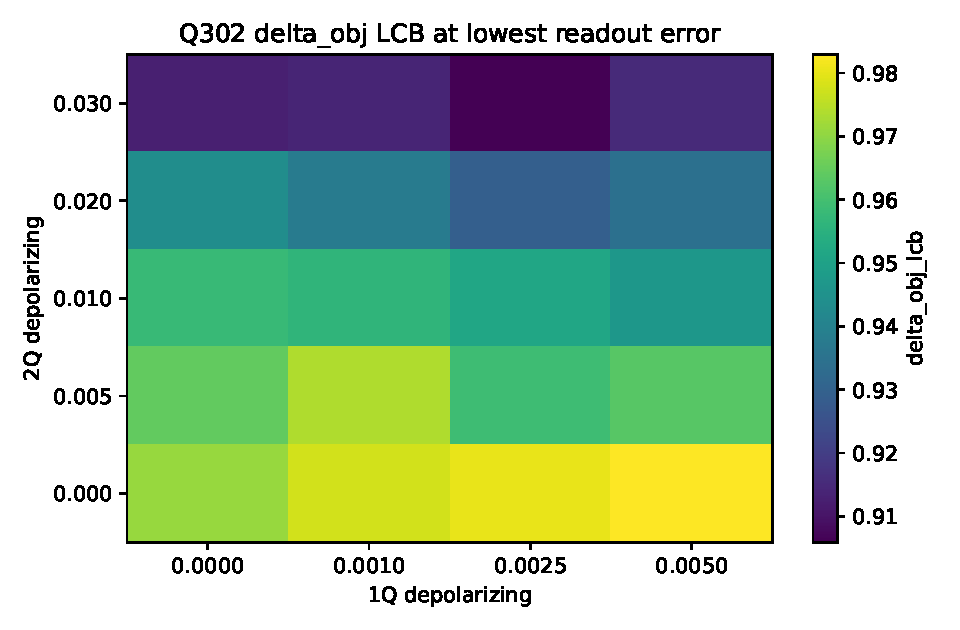
\includegraphics[width=\textwidth]{fig_q302_noise_readiness.pdf}
\caption{Q302 local readiness sweep before QPU execution.  The left panel shows
pass/fail status at the highest readout-flip setting in the sweep.  The right
panel shows the numerical margin over the preregistered thresholds at that same
readout setting.  The hardware run is interpreted only after theory, local
simulation, preregistration, and raw analysis gates have passed.}
\end{figure}

\section{Claim Discipline}

A601 records ten claims, zero unsupported claims, and two Q-grade hardware
illustration claims.  The final artifact route is
\texttt{foundations\_artifact\_with\_bounded\_quantum\_illustration}: the
theory package is supported, and the hardware observation is eligible only as a
bounded quantum illustration.

\begin{table}[htbp]
\centering
\begin{tabularx}{\textwidth}{@{}P{0.2\textwidth}Y@{}}
\toprule
Positive claim & Boundary \\
\midrule
Basis-order-orientation separation &
Supported by proofs, exact checks, and counterexamples. \\
Record capacity and no-go package &
Supported independently of QPU data. \\
IBM hardware result &
Supports a bounded four-qubit GHZ illustration only. \\
\bottomrule
\end{tabularx}
\caption{Allowed positive interpretations.}
\end{table}

\begin{table}[htbp]
\centering
\begin{tabularx}{\textwidth}{@{}P{0.28\textwidth}Y@{}}
\toprule
Rejected interpretation & Reason \\
\midrule
Basis uniqueness as the main novelty &
This is imported context under fixed-partition assumptions. \\
Hardware proof of the theorem package &
The theory and no-go results are established upstream of H501. \\
Orientation from redundancy alone &
Orientation-swap examples remain valid without an anchor. \\
Mitigation replacing raw analysis &
H503 is secondary and cannot override H502. \\
\bottomrule
\end{tabularx}
\caption{Explicit negative interpretations frozen by A602.}
\end{table}

\section{Reproducibility}

The frozen reproducibility archive is
\path{objective-clocks-reproducibility.tar.gz}.  Its SHA-256 is recorded
outside the archive payload in
\path{results/processed/A603_reproducibility_manifest.json} and
\path{docs/FINAL_DECISION.md}.  This avoids embedding the archive hash inside
files that are themselves archived.  The A603 manifest records the archived
file set, source commit, a successful clean reproduction run, and no recorded
secret values.  The clean reproduction command was:
\[
  \texttt{python scripts/reproduce\_all.py}
\]
The recorded terminal tail ends with 55 passing tests.  The public repository
also includes \path{CITATION.cff}; until a manuscript is released, the artifact
should be cited by title, author, repository URL, frozen tag, and the manifest
archive hash.

\section{Limitations}

The artifact is intentionally small in hardware scale.  The IBM run is a
four-qubit illustration of the GHZ/dephased-control workflow, not a many-body
demonstration of objective histories.  The theoretical claims depend on the
specified record model and admissible partitions.  The report does not solve
partition-independent Hilbert-space factorization or derive an orientation
anchor from redundancy alone.  Those remain outside the claim boundary.

\appendix
\section{Three-Round Review Record}

The final report and README were reviewed through four roles across three
rounds.  The review was performed as an internal artifact audit rather than as
peer review.

\begin{longtable}{@{}P{0.13\textwidth}P{0.18\textwidth}P{0.31\textwidth}P{0.29\textwidth}@{}}
\toprule
Round & Reviewer role & Challenge & Resolution \\
\midrule
\endhead
1 & Conceptual reviewer &
The README and report could overstate basis uniqueness as novelty. &
Moved fixed-partition basis uniqueness to related-work context and made the
basis-order-orientation separation the central claim. \\
1 & Mathematical reviewer &
Linear extensions might be mistaken for physical histories. &
Promoted the chain criterion and diamond counterexample to the core result. \\
1 & Hardware reviewer &
The IBM result could be read as proof of the theory. &
Labeled H501 as a bounded illustration and kept raw H502 as primary. \\
1 & Reproducibility reviewer &
The artifact needed a direct archive/hash story. &
Added the archive SHA-256, source commit, file count, and reproduction command. \\
\midrule
2 & Conceptual reviewer &
Non-specialists need vocabulary before the tables. &
Added a concept-primer table before technical evidence. \\
2 & Mathematical reviewer &
The orientation no-go boundary needed explicit wording. &
Added orientation-anchor language to the abstract, primer, and limitations. \\
2 & Hardware reviewer &
Backend amendment provenance could look like post-result selection. &
Documented the cancelled queued Marrakesh job as pre-result provenance and
identified Kingston as the only completed observation. \\
2 & Reproducibility reviewer &
Operational details should not dominate the scientific changelog. &
Moved changelog wording toward scientific chronology and left low-level details
to manifests and docs. \\
\midrule
3 & Conceptual reviewer &
The motivation should explain why clocks require more than objectivity. &
Rewrote the opening around agreement on alternatives versus agreement on a
physical history. \\
3 & Mathematical reviewer &
Capacity and no-go claims needed evidence-file pointers. &
Added T101, T103, C2, C3, C4, and C5 references in the methods narrative. \\
3 & Hardware reviewer &
Mitigation status needed stronger guardrails. &
Stated that H503 cannot rescue or replace H502. \\
3 & Reproducibility reviewer &
Figures needed visual-context justification. &
Included the tracked publication figures and described what each one supports. \\
\bottomrule
\end{longtable}

\bibliographystyle{plain}
\bibliography{research_artifact_references}

\end{document}
